\chapter{$D_s \rightarrow K$ and $B_s \rightarrow K$ form factors}\label{cha:DsBstoK}

\section{Correlator fitting}\label{sec:HsK_corr_priors}

\subsection{Priors}\label{sec:HsK_priors}

\begin{table*}
\caption{Parameters and statistics related to the correlation functions generated from the gluon field ensembles used in this work.  Column 2 gives the number of correlator configurations $N_\mathrm{cfg}$ times the number of sources $N_\mathrm{src}$ for given ensemble.  Column 3 gives the range of heavy quark masses (in lattice units), where the lightest option is chosen to be tuned to the physical charm quark mass.  Column 4 gives the non-zero twist angles $\theta\neq0.0$, which relate to three-momentum via equation \ref{eq:twist_angle}; we note that all ensembles also have correlators with values of $\theta=0$ as well.  Finally, column 5 gives the range of source-sink separation values $T$.  This table is identical to table \ref{tab:Hpi_Stats} in chapter \ref{cha:DBtopi}, as these parameters and statistics apply to both the $H\rightarrow\pi$ and $H_s\rightarrow k$ meson decays}
\begin{center} 
\begin{tabular}{l c c c c}
\hline
      Set & $N_{\mathrm{cfg}}\times N_{\mathrm{src}}$ & $am_h$ & $\theta\neq0.0$ & $T$ \\
\hline
\hline
    1 - f5   &$500 \times 16$  & 0.450, 0.55, 0.675, 0.8 &  0.4281, 1.282, 2.1410, 2.570 & 15, 18, 21, 24 \\
\hline
    2 - fphys   & $500 \times 8$& 0.433, 0.555, 0.678, 0.8 &  0.58, 0.87, 1.13, 3.000 & 15, 18, 21, 24 \\
\hline
        3 - sf5 & $500 \times 8$& 0.274, 0.5, 0.65, 0.8 &  1.261, 2.108, 2.666, 5.059 & 22, 25, 28, 31 \\
\hline
    4- sfphys &$100 \times 4$& 0.2585, 0.5, 0.65, 0.8 &  2.522, 4.216, 7.94, 10.118 & 22, 25, 28, 31 \\
\hline
    5 - uf5 & $375 \times 4$& 0.194, 0.4, 0.6, 0.8 & 0.706, 1.529, 2.235, 4.705 & 29, 34, 39, 44 \\
\hline
\hline
\end{tabular}
\end{center}
\label{tab:HsK_Stats}
\end{table*}


\begin{table}[]
    \centering
    \caption{Fractional uncertainties given to priors for ground state meson masses $\Delta(M)$ and amplitudes $\Delta(A)$.  Heavy-strange meson amplitude fractional uncertainties $\Delta(M_{H_s})$ apply only to the lightest $H_s$ meson option on each ensemble.  The ratio $R(\nicefrac{A_3}{A_0})$ is used in equation \ref{eq:Hmeson_amp_scaling} to determine the fractional uncertainties of of the heavier $H_s$ meson amplitude priors. $\Delta(A^*)$ is the fractional uncertainty given to all oscillating and or non-ground state amplitude priors.}
    \begin{tabular}{c c c c c c c}
    \hline
    Ensemble & $\Delta(M_K)$ &  $\Delta(M_{H_s})$  & $\Delta(A_K)$ & $\Delta(A_{H_s})$ &  $R(\nicefrac{A_3}{A_0})$ & $\Delta(A^*)$\\
    \hline
    f5  & 0.02 & 0.05 &  0.03 & 0.11 & 2.0 & 5.0\\
    fphys & 0.02 & 0.05 & 0.03 & 0.22 & 2.0 & 6.1\\
    sf5 & 0.05 & 0.05 & 0.08 & 0.10 & 4.0 & 2.6\\
    sfphys & 0.05 & 0.10 & 0.15 & 0.65 & 2.0 & 2.0\\
    uf5 & 0.10 & 0.05 & 0.15 & 0.20 & 4.0 & 2.0\\
    \hline
    \end{tabular}
    \label{tab:HsKmeson_mass_and_amp_priors}
\end{table}

\begin{table}[]
    \centering
    \caption{$Hs\rightarrow K$ ground state three-point amplitude priors $P[J_{00}^{nn}]$ for all ensembles, twists $\theta$, and currents $J \in \{S,V^0,V^1,T\}$.  Twist is related to the kaon's three-momentum $\vec{p}$ via equation \ref{eq:twist_angle}.  Methods for determining these priors is discussed in section \ref{sec:Amp_effs_3pt}.}
    \label{tab:3ptpriors_HsK}
    \begin{tabular}{c c | c c c c}
    \hline
    \hline
    Ensemble & $\theta$ & $S$ & $V^0$ & $V^1$ & $T$ \\
    \hline
    \hline
    f5 & 0.0    & 1.8(1.8)   & 0.8(0.8)   & -          & -   \\
       & 0.4281 & 1.75(1.75) & 0.75(0.75) & 0.1(0.1)   & 0.07(0.07) \\
       & 1.282  & 1.35(1.35) & 0.6(0.6)   & 0.2(0.2)   & 0.12(0.12) \\
       & 2.1410 & 1.0(1.0)   & 0.5(0.5)   & 0.22(0.22) & 0.14(0.14) \\
       & 2.570  & 0.85(0.85) & 0.5(0.5)   & 0.3(0.3)   & 0.15(0.15)\\
    \hline
    fphys & 0.0   & 1.90(1.90) & 1.0(1.0)   & -          & -         \\
          & 0.58  & 1.75(1.75) & 0.9(0.9)   & 0.1(0.1)   & 0.05(0.05) \\
          & 0.87  & 1.75(1.75) & 0.85(0.85) & 0.12(0.12) & 0.08(0.08) \\
          & 1.13  & 1.75(1.75) & 0.8(0.8)   & 0.15(0.15) & 0.1(0.1) \\
          & 3.000 & 1.25(1.25) & 0.6(0.6)   & 0.2(0.2)   & 0.15(0.15) \\
          & 5.311 & 0.5(0.5)   & 0.3(0.3)   & 0.15(0.15) & 0.1(0.1)\\
    \hline
    sf5   & 0.0   & 2.0(2.0) & 1.0(1.0)   & -          & - \\
          & 1.261 & 1.5(1.5) & 0.75(0.75) & 0.25(0.25) & 0.2(0.2)\\ 
          & 2.108 & 1.2(1.2) & 0.6(0.6)   & 0.3(0.3)   & 0.2(0.2)\\ 
          & 2.666 & 1.0(1.0) & 0.6(0.6)   & 0.3(0.3)   & 0.2(0.2)\\ 
          & 5.059 & 1.0(1.0) & 0.75(0.75) & 0.25(0.50) & 0.2(0.2)\\
    \hline
    sfphys & 0.0    & 2.0(2.0)   & 1.25(1.25) & -          & - \\
           & 2.522  & 1.5(1.5)   & 0.9(0.9)   & 0.25(0.25) & 0.15(0.15)\\ 
           & 4.216  & 1.25(1.25) & 0.75(0.75) & 0.3(0.3)   & 0.2(0.2) \\
           & 7.94   & 1.0(1.0)   & 0.5(0.5)   & 0.25(0.25) & 0.2(0.2) \\
           & 10.118 & 1.0(1.0)   & 0.5(1.0)   & 0.2(0.4)   & 0.2(0.3)\\
    \hline
    uf5 & 0.0   & 2.0(2.0)   & 1.25(1.25) & -        & - \\
        & 0.706 & 1.75(1.75) & 1.0(1.0)   & 0.2(0.2) & 0.15(0.15)\\ 
        & 1.529 & 1.5(1.5)   & 0.75(0.75) & 0.3(0.3) & 0.20(0.2) \\
        & 2.235 & 1.0(1.0)   & 0.6(0.6)   & 0.3(0.3) & 0.20(0.2) \\
        & 4.705 & 1.0(1.0)   & 0.5(1.0)   & 0.3(1.0) & 0.2(0.5)\\
    \hline
    \hline
    \end{tabular}
\end{table}


\begin{table}
  \caption{$H_s\rightarrow K$ prior absolute uncertainties for all ensembles, for all oscillating and or non-ground state fit parameters $J_{ij}^{kl} \neq J_{00}^{oo}$, for $J\in \{S,V^0,V^1,T\}$.  The notation $J_{\neq0}$ indicates the values used to assign priors to all higher order exponential states $J_{ij\neq00}^{kl}$. The notation $J_{\mathrm{osc}}$ indicates the values used to assign priors to all lowest lying oscillating states $J_{00}^{kl\neq nn}$. Central values given to all associated priors are equal to 0.0. A special prior uncertainty scaling term $\sigma_\mathrm{ens}$ for each ensemble is given in final column.  The scaling term applies to select non-ground state three point amplitudes $J_{00}^{on}$ and $J_{10}^{kl}$ for all $k,l \in \{n,o\}$.}
  \begin{center} 
    \begin{tabular}{c c c c c c c c c c}
    \hline
    \hline
    Ensemble & $S_{\neq 0}$ & $S_{\mathrm{osc}}$ & $V^0_{\neq 0}$ & $V^0_{\mathrm{osc}}$ & $V^1_{\neq 0}$ & $V^1_{\mathrm{osc}}$ & $T_{\neq 0}$ & $T_{\mathrm{osc}}$ & $\sigma_\mathrm{ens}$\\
    \hline
    \hline
    f5 & 0.43 & 1.1 & 0.75 & 2.0 & 0.12 & 1.0 & 0.8 & 1.0 & 1.8\\
    fphys & 0.42 & 1.52 & 1.0 & 3.3 & 0.11 & 0.2 & 0.06 & 0.22 & 2.2\\
    sf5 & 0.24 & 0.55 & 0.26 & 0.86 & 0.1 & 0.25 & 0.01 & 0.3 & 4.0\\
    sfphys & 0.2 & 0.4 & 0.25 & 2.0 & 0.07 & 0.14 & 0.08 & 0.16 & 5.5\\
    uf5 & 0.16 & 0.4 & 0.25 & 0.20 & 0.07 & 0.21 & 0.06 & 0.15 & 5.0\\
    \hline
    \hline
    \end{tabular}
    \end{center}
  \label{tab:3pt_pesky_priors_HsK}
\end{table}

\subsection{Results}\label{sec:HsK_results}
\begin{figure}
    \centering
    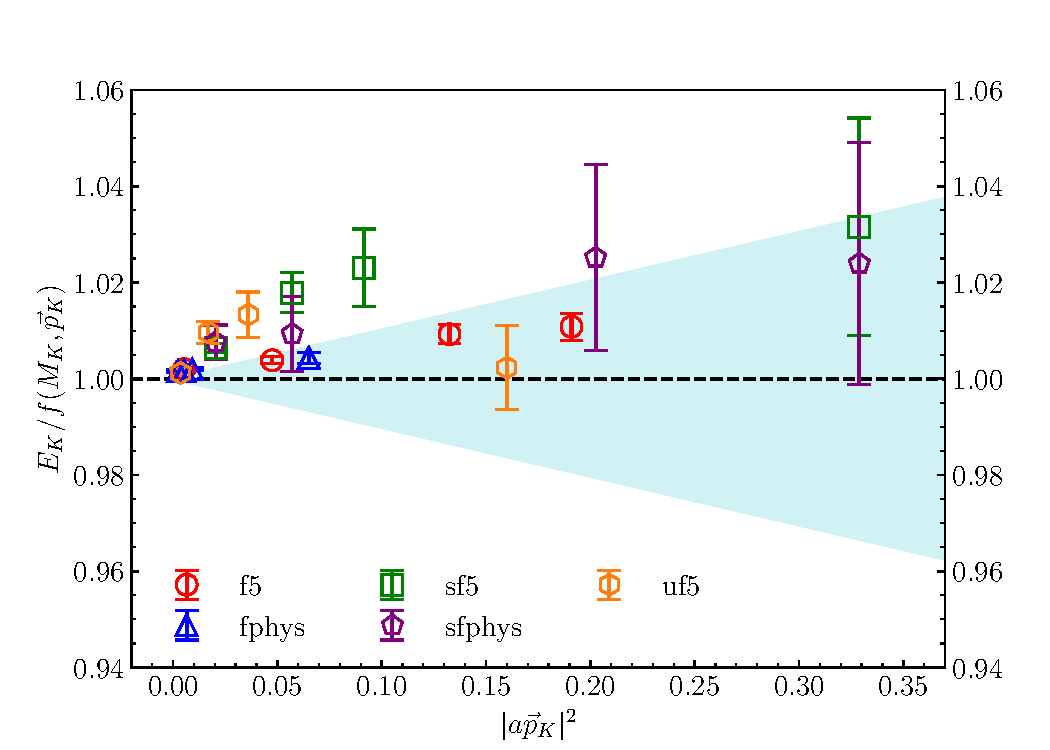
\includegraphics[width=0.8\linewidth]{chapter7/pdfs/customHsK_Edisp_plots.pdf}
    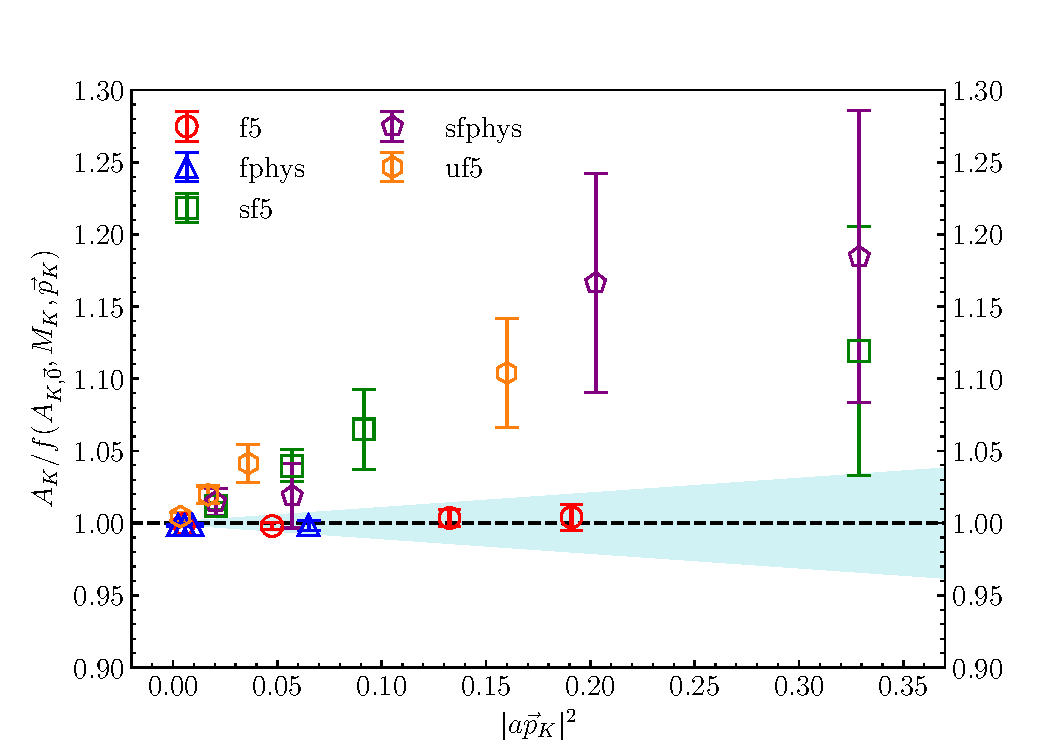
\includegraphics[width=0.8\linewidth]{chapter7/pdfs/customHsK_Ampdisp_plots.pdf}
    \caption{Energy (top) and amplitude (bottom) dispersion relation plots for current set of $H_s\rightarrow K$ correlator fits.  Data shown are ground state, non-zero twist energy and amplitude fit posteriors divided by a function equal to the right hand side of either equation \ref{eq:dispersion_energy} (energy) or equation \ref{eq:dispersion_amplitude} (amplitude) without the discretization factor.  The shaded cyan corresponds to the area bound by the function $y=1\pm \left(\frac{a\vec{p}}{\pi}\right)^2$.}
    \label{fig:HsK_disp-plots}
\end{figure}

\section{$z$-expansion fit}\label{sec:Hsk_zfit}

\subsection{Priors}\label{sec:HsK_zfit_priors}

\subsection{Results}\label{sec:HsK_zfit_results}

\section{Status of form factors calculations}\label{sec:HsK_FF_status}

\subsection{$D_s\rightarrow K$}\label{sec:BsK_status}

\subsection{$B_s \rightarrow K$}\label{sec:BsK_status}